\section{Experimental Evaluation}
This section will present some findings from the initial assessment of utilizing Petal and its impact on the overall performance of the application. Multiple tests were conducted on various environments.
\subsection{Point-to-point Communications}

Ahmed et al. \cite{hoefler_case_2007} benchmarked a series of tests, which were transformed using Petal tool, including 1D heat decomposition, 2D heat decomposition  \cite{ahmed_petal_2016}, and DT from the NAS NPB 3.3 \cite{noauthor_nas_nodate}. 
The performance of the transformed application was evaluated by varying the number of MPI processes. In the case of 1D heat, the number of MPI processes ranged from 6 to 200 tasks. 
For 2D heat and DT with classes W (Class W: workstation size - a 90's workstation; now likely too small) and A (standard test problems; ~4X size increase going from one class to the next), the number of MPI processors (NP) varied between 16 and 256. 
The results, depicted in \autoref{fig:p2p-benchmark}, demonstrate the execution time speedup 
$S = T_{\text{original}}/T_{\text{transformed}}$ achieved through the application of non-blocking transformation and the addition of persistent communication.
where $T_{\text{original}}$ is the the time needed to executed code before the transformation with Petal and $T_{\text{transformed}}$ is the execution time of the code after Petal substituted blocking communication with non-blocking or persistent one.
Analyzing the execution time of the original and transformed codes provides valuable information regarding the potential performance improvement achieved through the transformation. A ratio of $S = 1$ indicates no speedup. A ratio $S < 1$ implies that the transformed code performs worse, while a ratio of $S$ around 1 signifies a negligible performance gain.
The higher the value of $S$, the more performance gain can be achieved.\\

The experiments were conducted using the TACC Stampede System, which is a Dell Linux Cluster capable of processing 10 Petaflops (PF). 
The cluster consists of over 6400 Dell PowerEdge server nodes, each equipped with 32 GB of memory and 2 Intel Xeon E5 processors (Sandy Bridge, 8 cores). 
Additionally, the nodes are augmented with an Intel Xeon Phi Coprocessor (Knights Corner, 61 cores) using the MIC architecture.


\begin{figure}[!h]
    \centering
    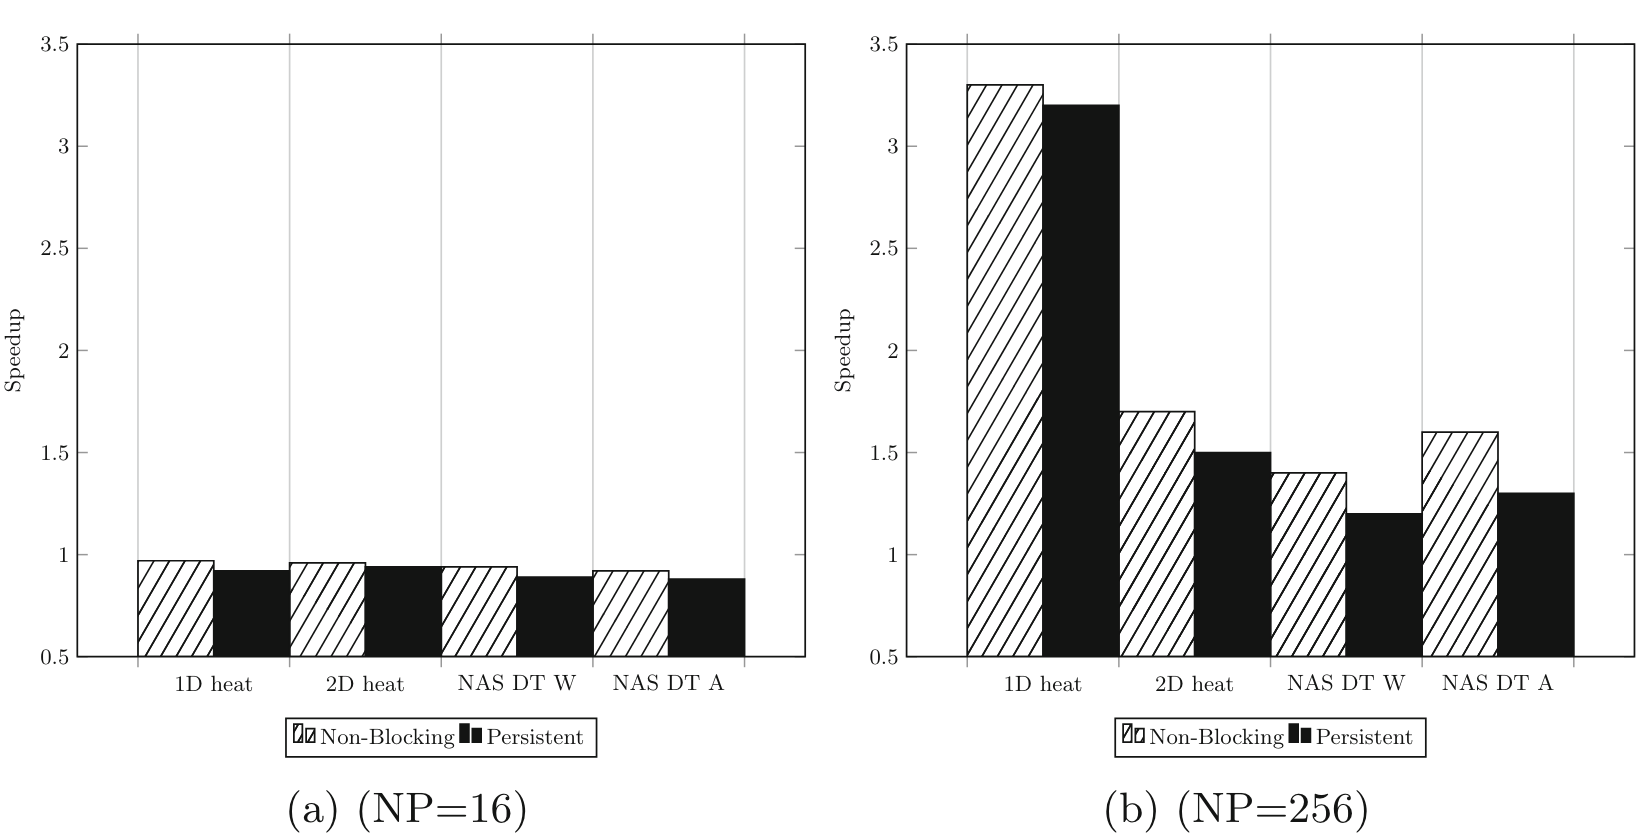
\includegraphics[width=\textwidth]{pictures/p2p-benchmark.png}
    \caption{Weak-scaling time speedup. \cite{ahmed_petal_2016}}
    \label{fig:p2p-benchmark}
\end{figure}
\autoref{fig:p2p-benchmark} provides a visual representation of the speedup achieved by the transformed code compared to the original code. The vertical axis represents the speedup, while the horizontal axis indicates the benchmarked problems.

When considering smaller programs and a smaller number of jobs, the speedup remains consistently below 1. This indicates that the benefit of non-blocking improvements is negligible and can sometimes even introduce overhead, resulting in worse performance.

However, significant performance improvements are observed with the non-blocking technique, with some cases showing increases of up to 30\%, such as in the NAS DT class A example with 256 processes. 
These improvements are consistently evident across all the transformed codes, showcasing their effectiveness as the problem size and the number of MPI tasks increase.
\subsection{Collective Communications}
Ahmed et al. \cite{ahmed_transforming_2017} conducted a performance comparison between the original code and the transformed code that employed nonblocking collectives.

The first test uses a C version of a benchmark code discussed by James Tullos \cite{Tullos_2014}. 
There is a code kernel consisting of three arrays, which are spread across multiple ranks. 
In this kernel, the first array is averaged, and the resulting value is utilized to make modifications to the second array. 
The minimum and maximum values in the second array are identified and employed, along with the sum of the first array, to modify the third array. 
Afterwards, the third array is reduced to a single sum that encompasses all ranks.\\
In the implementation of Ahmed \cite{ahmed_transforming_2017}, the kernel operates on three arrays \texttt{sub\_arr1}, \texttt{sub\_arr2} and \texttt{sub\_arr3} that are distributed across the processes. 
It uses \texttt{MPI\_Allreduce} to compute the average of the first array.
Using the average to compute new entries for the second array. 
The next step computes the global minimum and maximum values of the second array by two \texttt{MPI\_Allreduce} operations. (line 6-7)
The last step adds the average of the first array to all elements in the second array and uses the global min and max values to update the entries of the third array (line 9 - 12).
A last call to \texttt{MPI\_Allreduce} computes the sum of the third array (last line).

The number of MPI processes was varied  from 16 to 128, and tested with different message sizes, ranging from 16K to 524K with 16 processes, and from 65K to 4M with 128 processes.
\autoref{fig:intel-benchmark} demonstrates the execution time speedup ($S = T_{\text{original}}/T_{\text{transformed}}$) achieved through the application of non-blocking transformation with Petal.

Another benchmark was performed for conjugate gradient \autoref{collective_non-blocking}, which was discussed on Section \ref{sssec:collective_communication}. 
\autoref{fig:conj-benchmark} shows the speedup of transformed non-blocking version and non-blocking persistent version in comparison to application with blocking communications.

The tests were performed on a system with the following configuration:
LLNL cab cluster with 1,296 nodes with 16 core and 32GB memory each node, Intel Xeon E5-2670. 
The nodes are interconnected by InfiniBand in QDR mode. Openmpi-gnu-2.0.0 MPI with the default settings was applied for these tests.

\begin{figure}[!ht]
    \centering
    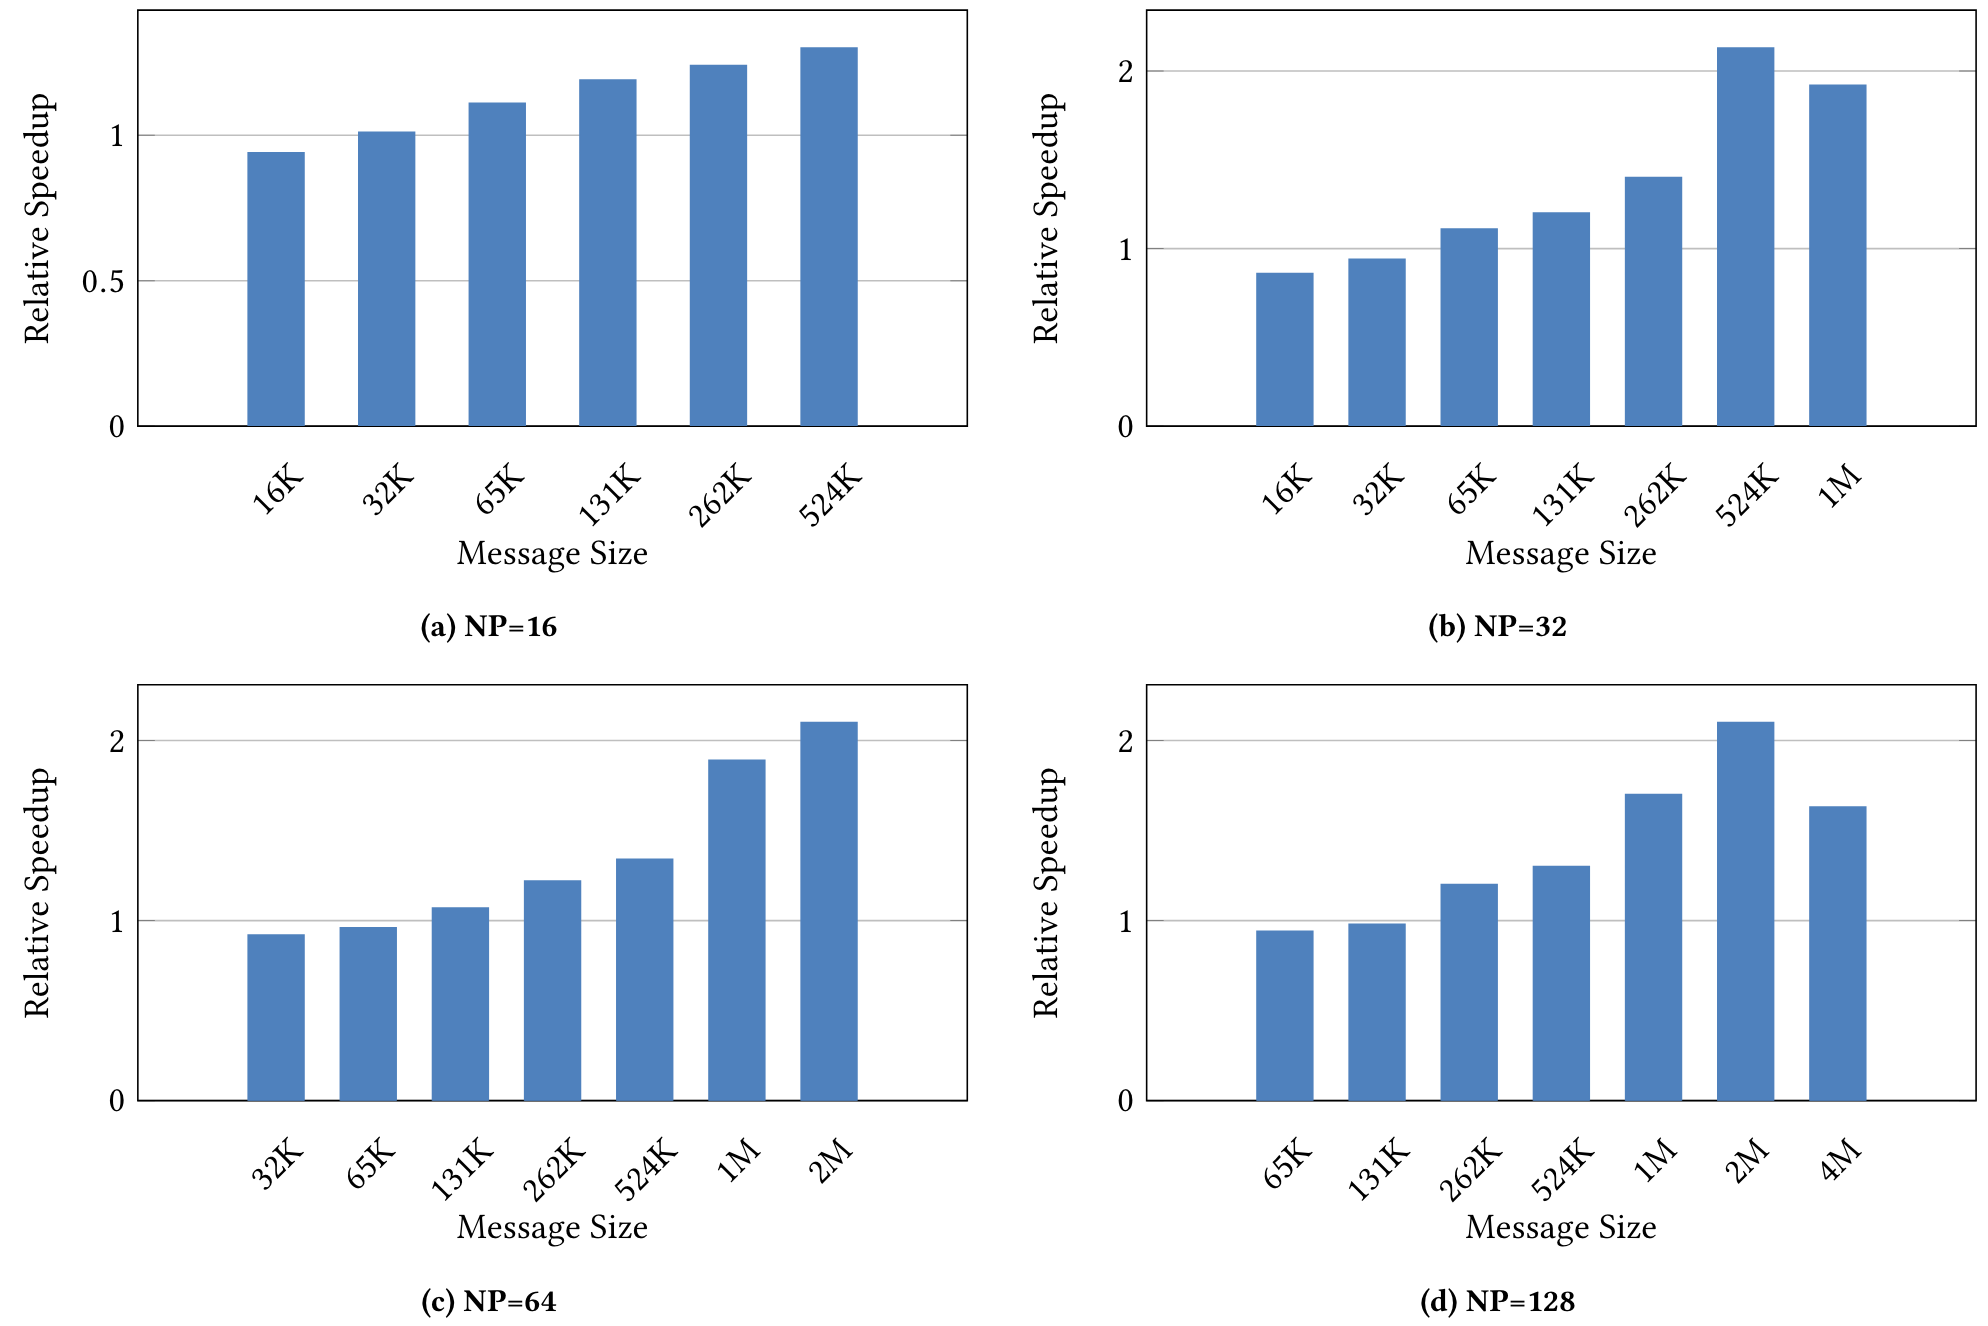
\includegraphics[width=\textwidth]{pictures/intel-benchmark.png}
    \caption{Weak-scaling for Intel benchmark. \cite{ahmed_transforming_2017}}
    \label{fig:intel-benchmark}
\end{figure}

\autoref{fig:intel-benchmark} illustrates the compwarative acceleration achieved by the nonblocking version in relation to the original code.
When utilizing 32 processes, enhancements are observed for message sizes exceeding 32K.
However, as the number of processes increases, the message threshold rises to 64K, 131K, and 262K, respectively, before the positive impact of nonblocking collectives becomes evident.
This phenomenon may be attributed to the relatively brief duration of overlapped computation compared to communication.
Under optimal circumstances, the nonblocking primitives achieve a twofold speedup compared to their corresponding blocking counterparts.
One of the potential factors contributing to this behavior is the utilization of cache.

\begin{figure}[!h]
    \centering
    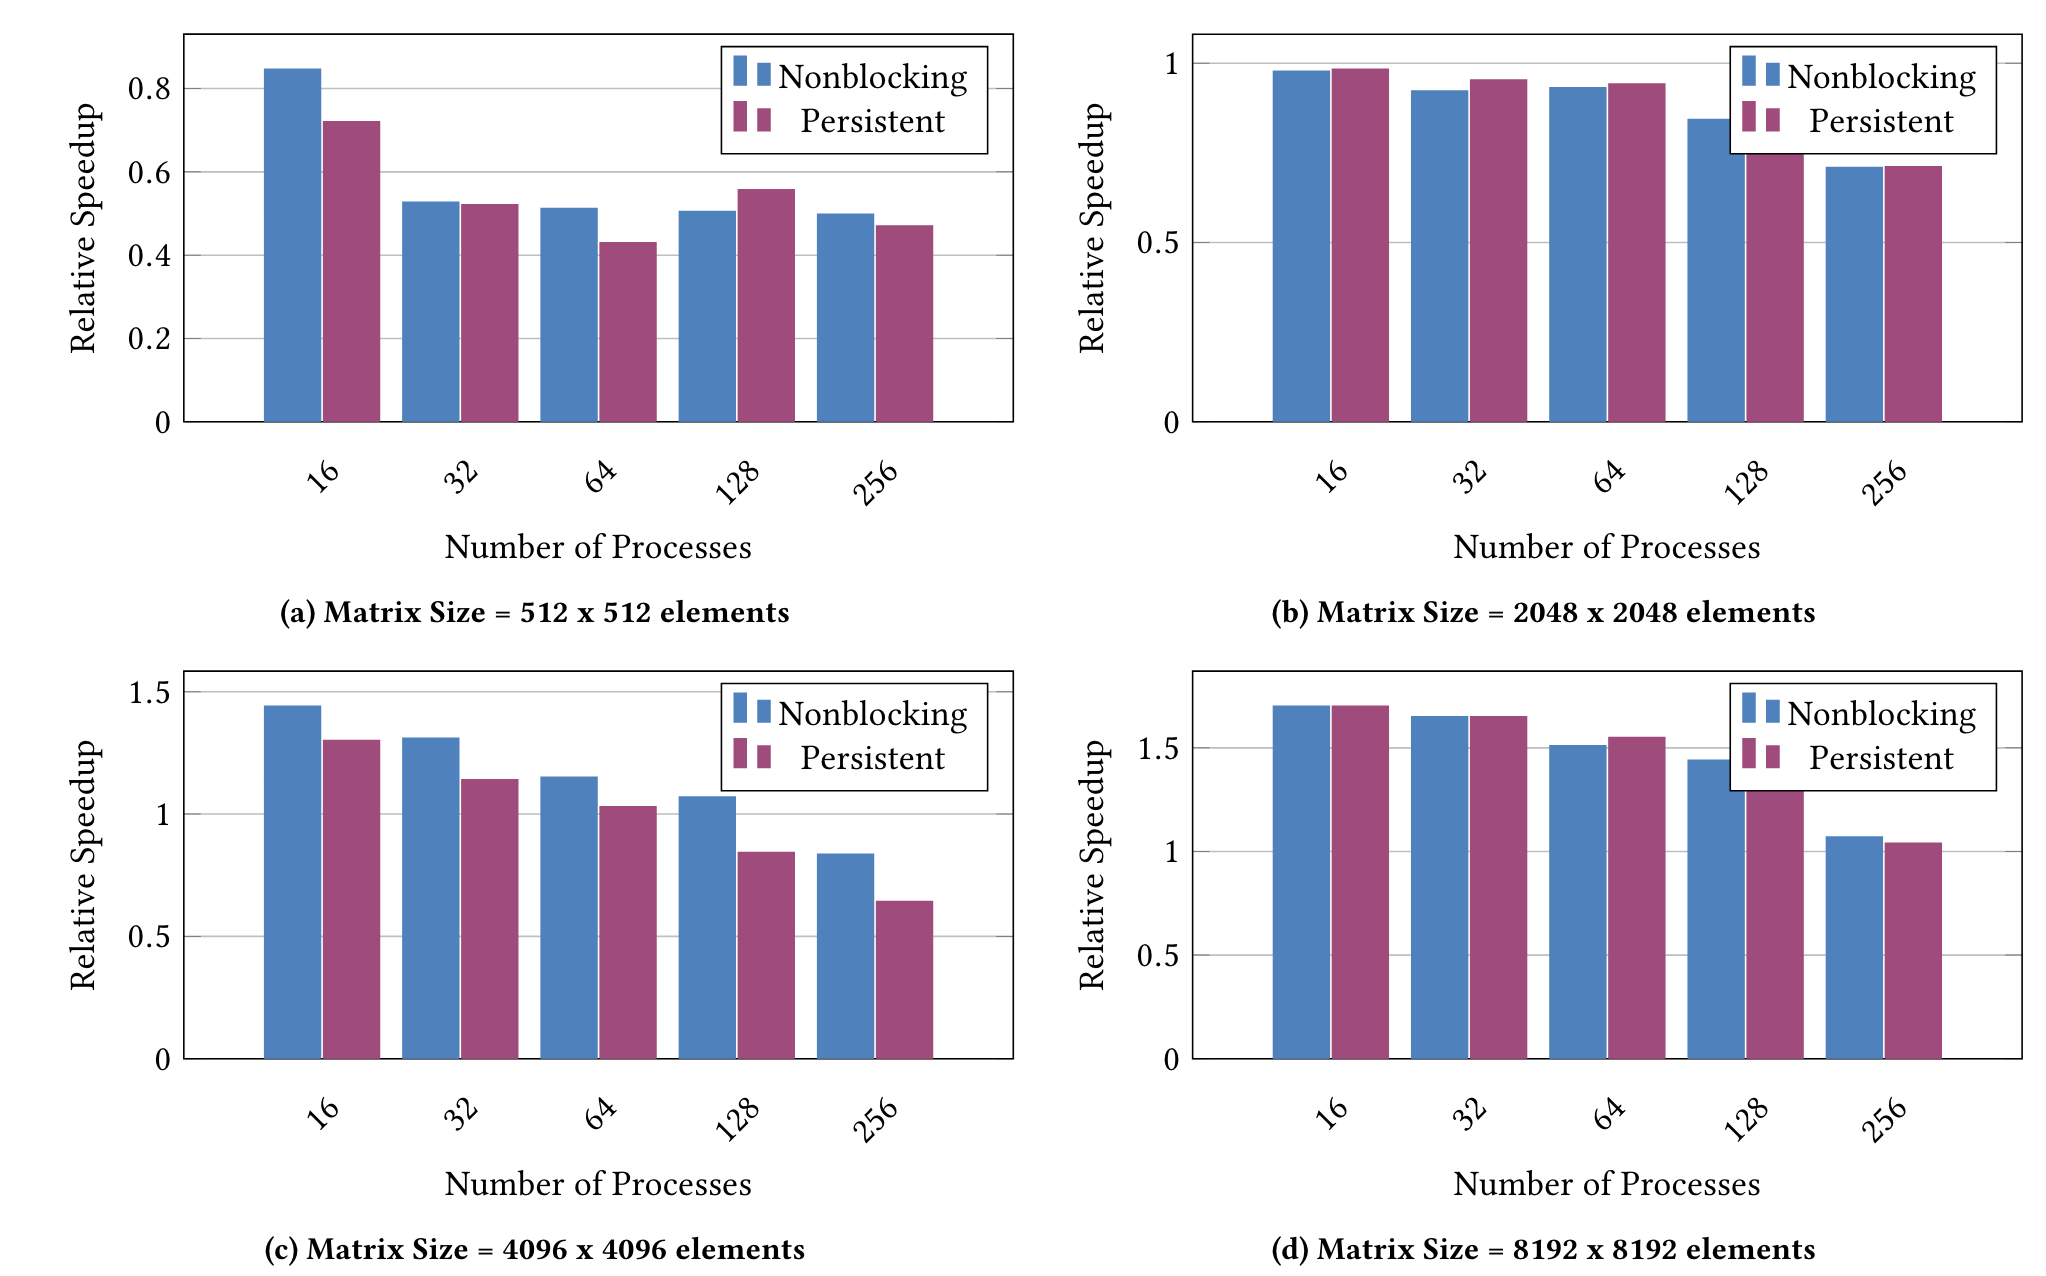
\includegraphics[width=\textwidth]{pictures/conj-benchmark.png}
    \caption{Weak-scaling for conjugate gradient benchmark.}
    \label{fig:conj-benchmark}
\end{figure}

For the conjugate problem \autoref{fig:conj-benchmark}, as the problem size increases, it becomes evident that the nonblocking version outperforms the blocking version. 
Nevertheless, with a higher number of processes, the benefits of using nonblocking operations diminish. 
This is primarily due to a reduction in the number of elements exchanged as the process count rises. 
Moreover, when dealing with extremely large matrix sizes, the conjugate gradient code for blocking collectives failed to complete within the allocated time on the machine, whereas the nonblocking version successfully finished. 
Ahmed et al. also implemented a transformation to persistent communication, which was not further explained in this paper. However, according to Ahmed et al., these transformations did not obtain any speedup improvement over its nonblocking counterparts.



